

\documentclass{beamer}
\usepackage{amsmath}
\usepackage{multirow}
\usepackage{booktabs}


% You can uncomment the themes below if you would like to use a different
% one:
%\usetheme{AnnArbor}
%\usetheme{Antibes}
%\usetheme{Bergen}
%\usetheme{Berkeley}
%\usetheme{Berlin}
%\usetheme{Boadilla}
%\usetheme{boxes}
%\usetheme{CambridgeUS}
%\usetheme{Copenhagen}
%\usetheme{Darmstadt}
%\usetheme{default}
%\usetheme{Frankfurt}
%\usetheme{Goettingen}
%\usetheme{Hannover}
%\usetheme{Ilmenau}
%\usetheme{JuanLesPins}
%\usetheme{Luebeck}
\usetheme{Madrid}
%\usetheme{Malmoe}
%\usetheme{Marburg}
%\usetheme{Montpellier}
%\usetheme{PaloAlto}
%\usetheme{Pittsburgh}
%\usetheme{Rochester}
%\usetheme{Singapore}
%\usetheme{Szeged}
%\usetheme{Warsaw}


\makeatother
\setbeamertemplate{footline}
{
  \leavevmode%
  \hbox{%
  \begin{beamercolorbox}[wd=.3\paperwidth,ht=2.25ex,dp=1ex,center]{author in head/foot}%
    \usebeamerfont{author in head/foot}Ziying Yang
  \end{beamercolorbox}%
  \begin{beamercolorbox}[wd=.7\paperwidth,ht=2.25ex,dp=1ex,center]{title in head/foot}%
    \usebeamerfont{title in head/foot}\insertshorttitle\hspace*{3em}
    \insertframenumber{} / \inserttotalframenumber\hspace*{1ex}
  \end{beamercolorbox}}%
  \vskip0pt%
}
\makeatletter
\setbeamertemplate{navigation symbols}{}

\title{How Precise Does Document Scoring Need To Be?}


\author{\textbf{Ziying Yang}, Alistair Moffat, and Andrew Turpin}


\institute[Universities of Melbourne] % (optional, but mostly needed)
{
  \inst{}%
  University of Melbourne
}


\date{}


\subject{Master Project Presentation}

\begin{document}

\begin{frame}
  \titlepage
\end{frame}


\section{Introduction}
\begin{frame}{Background -- Batch Evaluation Technique}
\begin{block}{Question}
\\[0.3em]
\textit{Is IR System A demonstrably better than IR System B?}
\end{block}
\pause
\\[1em]
For each of system A and B\\[0.4em]
\begin{itemize}
  \item For each of a set of topics
  \begin{itemize}
    \item Compute the \alert{similarity score} relative to the topic for each document
    \item Generate a run in decreasing score order
    \item Evaluate the run via relevance judgments and an effectiveness metric
    \item Generate a \alert{run score} for that system and topic
  \end{itemize}
  \pause
  \item Aggregate run scores over the set of topics into a single \alert{system score}\\[1em] 
  %seemed as the overall performance quality of the system
\end{itemize}

We then compare system A and B using their system scores.
\end{frame}

\section{Ties}
\begin{frame}{How to Deal with Tied Similarity Scores?}

Effectiveness metrics use {\color{blue}ranks}, not {\color{blue}similarity scores}.\\[1.5em]

Ties: when more than two items receive the same similarity scores.\\[1.5em]

How should \alert{similarity score ties} be handled?\\[1.5em]
%explain what is ties

{\color{blue}Different orderings} of tied documents may lead to {\color{blue}different system scores}, and might influence the outcome of the experiment.
% \begin{itemize}
%   \item We evaluate TREC-8 runs to determine the impact of tied scores
%   \item Any permutation of tied documents ordering can be presented to the user.
%   %\item Possible treatments: Pick an arbitrary ranking? Order them by document ID?
% \end{itemize}
\end{frame}
\begin{frame}{How to Deal with Tied Similarity Scores?}
\uncover<1->{\begin{block}{Example}
\begin{tabular}{l|@{\hspace{1.5em}} *{7}{l@{\hspace{1.8em}}}}
\tabent{rank, $k$}
  & 1
      & 2
        & 3
        & 4
          & 5
                & 6
            & 7
\\
\hline
\tabent{document, $d_k$}
  & D
      & H
          & A
        & C
            & M
          & S
              & W
\\
\tabent{gain, $r_k$}
  & 0
      & 0
          & 1
        & 1
            & 0
          & 1
              & 1
\\
\tabent{similarity score}
  & 9.8
      & \alert{9.3}
          & \alert{9.3}
        & \alert{9.3}
            & {\color{blue}8.4}
          & {\color{blue}8.4}
              & 8.2
% \\
% \tabent{groups}
%   & \multicolumn{1}{@{}l}{$b_1{=}1$}
%       & \multicolumn{1}{@{}l}{$b_2{=}2$}
%           &
%         &
%             & \multicolumn{1}{@{}l}{$b_3{=}5$}
%           &
%               & \multicolumn{1}{@{}l}{$b_4{=}7$}
\end{tabular}
\end{block}}
\only<1>{
Divide the ranking of a run into \alert{groups} in which the documents have the same similarity score\\[3.2em]
%Denote \alert{$b_g$} as the beginning rank of the \alert{$g$th} group.
}
\uncover<2->{Possible methods for dealing with ties in the run:
\begin{itemize}
\uncover<2->{\item {\color{blue}Run Order}
  \only<2>{: ignore the similarity score, use the presented ordering. (RBP$0.5=0.211$)\\[4.5em]}\only<3->{(RBP$0.5=0.211$)}}
\uncover<3->{\item {\color{blue}External Tie-Break Rule}
  \only<3>{: re-order tied documents in each group using fixed ordering criterion, such as sorting by document ID (\texttt{trec\_eval} program), filename, length and so on. (RBP$0.5=0.227$)\\[3.2em]}\only<4->{(RBP$0.5=0.227$)} }

\uncover<4->{\item {\color{blue}Limits}
  \only<4>{: compute the best and worst run scores that may arise and present a score range instead of a single score value. (RBP$0.5 = [0.211,0.414]$)\\[3.2em]} \only<5->{(RBP$0.5 = [0.211,0.414]$)}}

\uncover<5->{\item {\color{blue}Averaging Across Permutations}
  \only<5>{: compute the average run score across all possible permutations of documents in each group. (RBP$0.5 = 0.323$)\\[3.2em]}}
\end{itemize}}
\end{frame}

\begin{frame}{Ties in TREC Experimentation}
To explore the role of ties in TREC evaluation, we re-sorted the TREC7 submissions, using decreasing {\color{blue}similarity score} as a {\color{blue}primary key}, and increasing {\color{blue}rank} as a {\color{blue}secondary key}.

\begin{table}
\caption{The percentage of \alert{103} systems, \alert{50 $\times$ 103} runs and \alert{4,900,042} documents affected by ties occurring in TREC7 Ad--Hoc runs after score-based re-sorting}
\begin{tabular}{l c ccc}
%\toprule
%  && \multicolumn{3}{c}{Percentage affected}
%\\
%\cmidrule{3-5}
  && systems
    & runs
      & documents
\\
\midrule
Tied similarity scores
  && 95.2\%
    & 91.0\%
      & 14.0\%
\\
Rank/score contradictions
  && \D6.8\%
    & \D4.2\%
      & \D1.4\%
\\
%\bottomrule
\end{tabular}
\end{table}
\end{frame}

\begin{frame}{Ties in TREC Experimentation}
Examine the effect of ties on AP scores for systems
\begin{itemize}
  \item For each system, calculate {\color{blue}mean AP} score over 50 topics using {\color{blue}\texttt{trec\_eval}}.
  \item Select the top 80 systems, as ordered by mean AP score.
  \item For each selected system, compute
  \begin{itemize}
    \item Run Order: {\color{blue}mean} (across topics) of the AP score (by {\color{blue}\texttt{trec\_eval}}).
    \item Limits: {\color{blue}mean} (across topics) of the {\color{blue}best} and {\color{blue}worst} AP score.
    \item Permuations: {\color{blue}mean} (across topics) of the {\color{blue}average} (across permutations of the tied groups in the run) AP score.
    
  \end{itemize}

\end{itemize}
\end{frame}

\begin{frame}{Imprecision in AP Scores Caused by Ties}
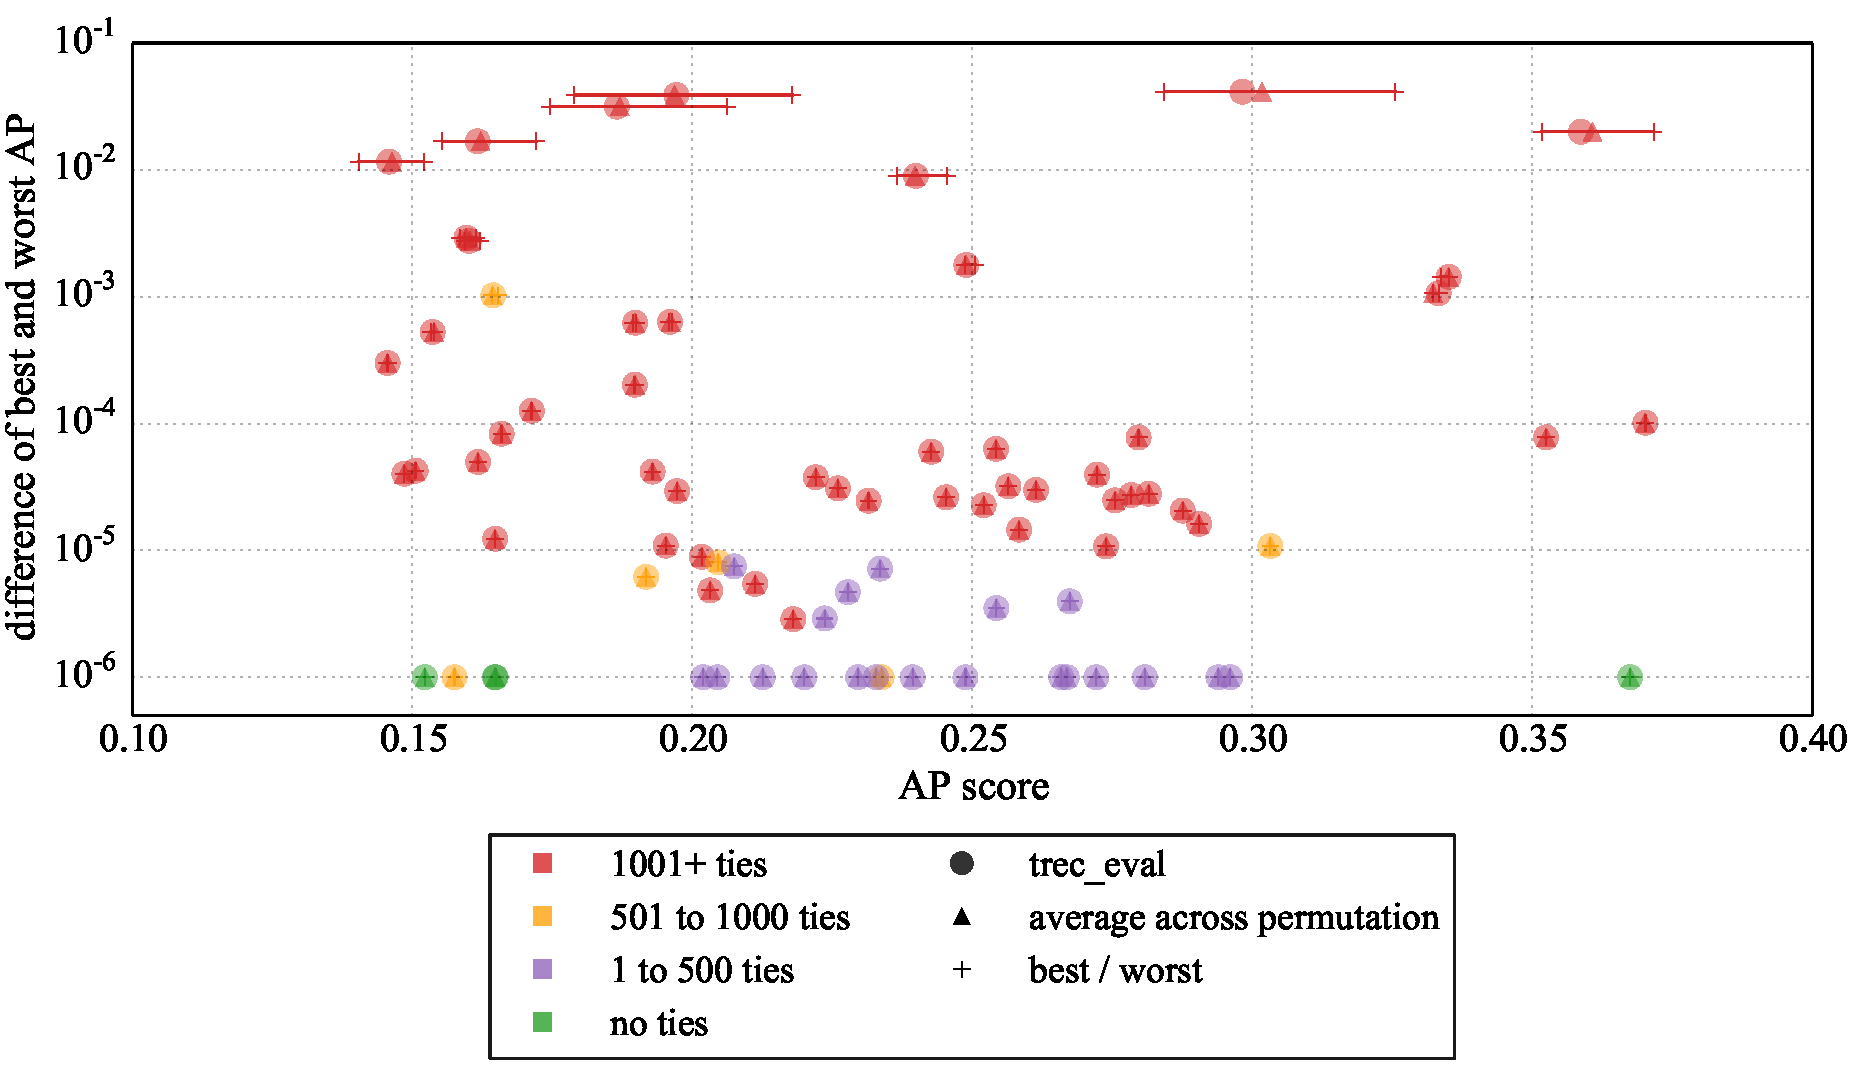
\includegraphics[width=0.98\textwidth]{figs/fig-trec7-ap-scores.pdf}
\end{frame}

\section{Deliberate Score Grouping}
\begin{frame}{Similarity Score Rounding}
%We showed that tied scores had the potential to be disruptive to TREC evaluation, but in practical turns did not. \\[1.5em]

Ties may have been caused by {\color{blue}similarity score rounding}. \\[1em]

\begin{block}{Question}
\textit{Do documents really need to assign similarity scores with high accuracy? How much similarity score rounding can be tolerated without greatly affecting system comparisons?}
\end{block}
\\[1em]
The finding offers the potential for {\color{blue}approximate scoring regimes} that provide {\color{blue}faster search} with little or no loss of effectiveness.

\end{frame}

\begin{frame}{Deliberate Similarity Score Grouping}
Will the deliberate use of ties affect retrieval quality?\\[1em]

Documents are scored and assigned in \alert{bands} of the ranking. Bands are defined geometrically based on a parameter \alert{$\rho$} ($\rho > 1$). More precisely:\\[0.5em]

For the \alert{$g$th} band:
\begin{itemize}
\item the begining rank: $b_g = \lceil{\rho\cdot b_{g-1}}\rceil$, $b_1 = 1$.
\item the ending rank: $e_g = b_{g+1}-1$\\[0.5em]
\end{itemize}
For example:\\
if \alert{$\rho = 2$}\\[0.3em] \text{ } 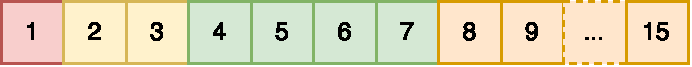
\includegraphics{figs/grouping_exp_rho2.pdf}\\
if \alert{$\rho=1.62$} (the golden ratio)\\[0.3em] \text{ } 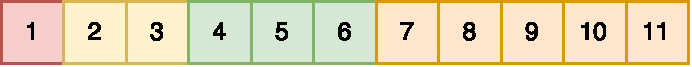
\includegraphics{figs/grouping_exp_rho162.pdf}
\end{frame}

%-----the run concept changed-----

\begin{frame}{Run Score Differences in Practice}
  For each of the $80 \times 50$ system--topic runs 
  \begin{itemize}
  \item compute effectiveness scores of metrics RR, RBP0.5, RBP0.85 and AP using the {\color{blue}original run}
  \item map original run to a banded ranking list using a $\rho$
  \item score the {\color{blue}banded run} using same metrics\\[1em]
  \end{itemize}
  Compute $80 \times 50$ run score differences.
\end{frame}


\begin{frame}{Variation in Run Score of AP}
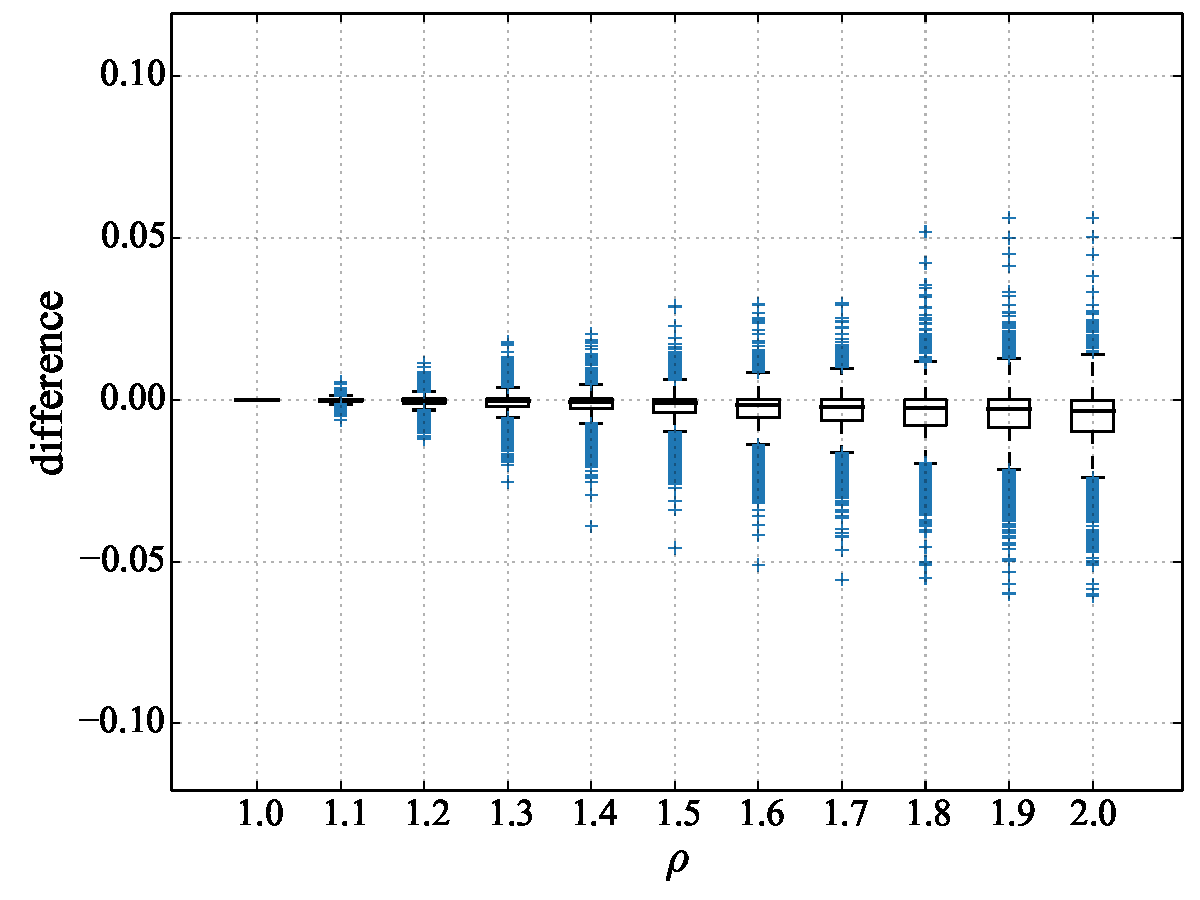
\includegraphics[width=0.9\textwidth]{figs/fig-score-variation-ap.pdf}
\end{frame}

\begin{frame}{Variation in Run Score of RBP ($p = 0.85$)}
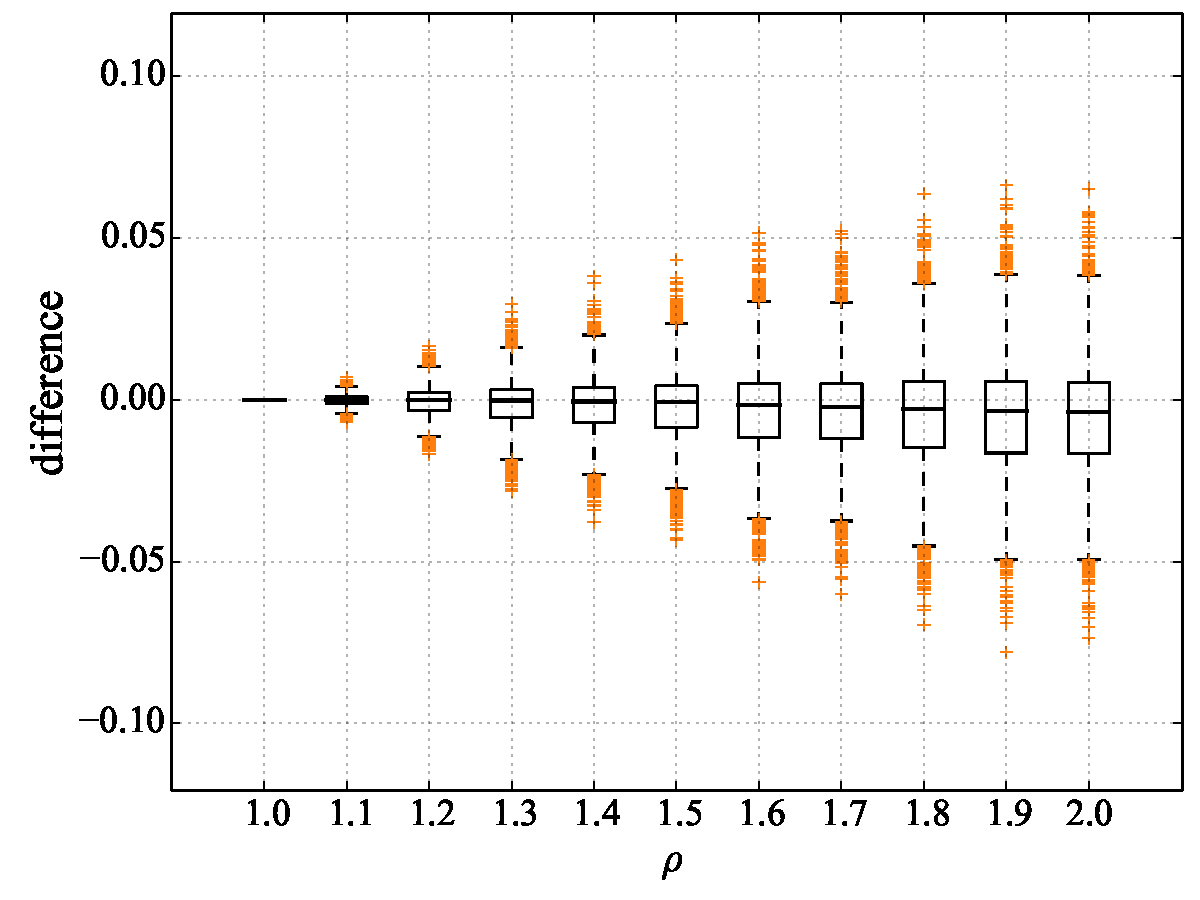
\includegraphics[width=0.9\textwidth]{figs/fig-score-variation-rbp85.pdf}
\end{frame}

\begin{frame}{Variation in Run Score of RBP ($p = 0.5$)}
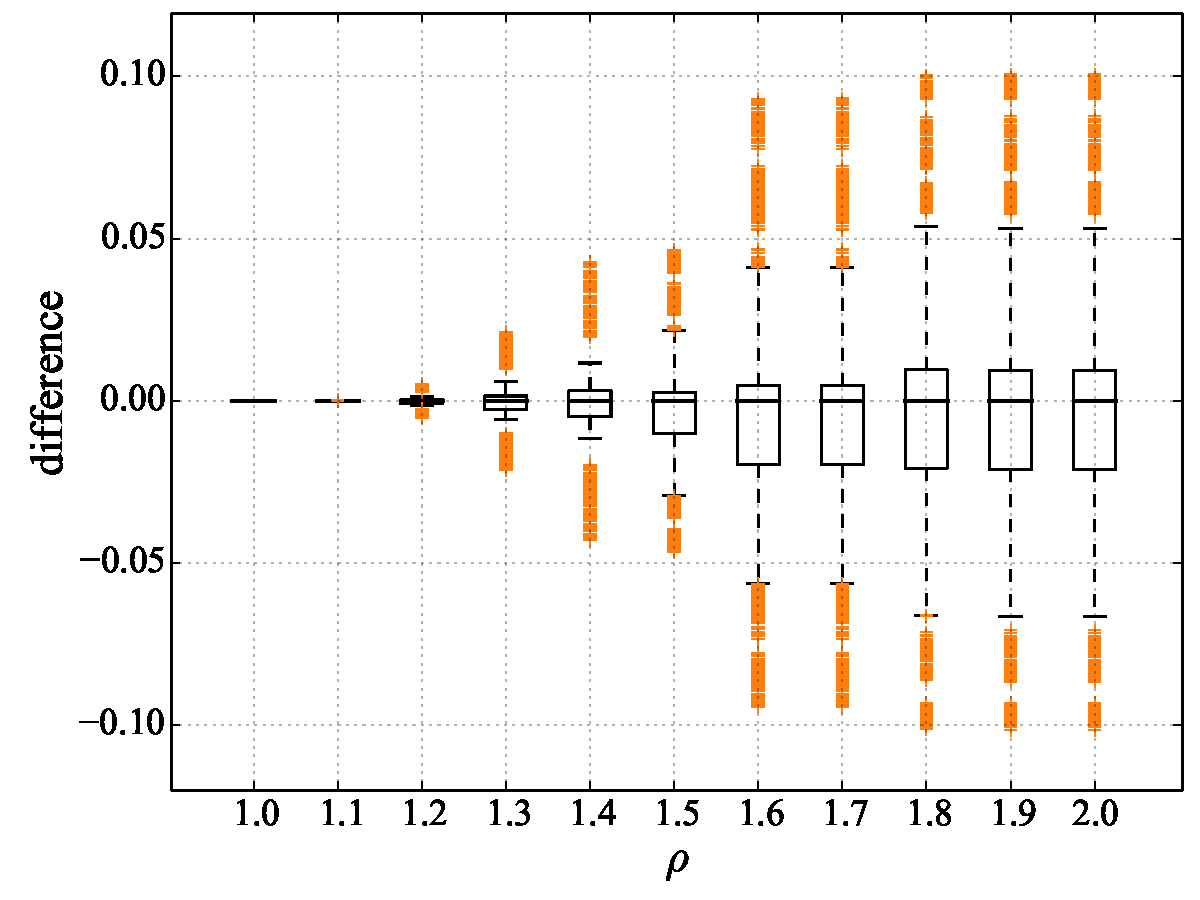
\includegraphics[width=0.9\textwidth]{figs/fig-score-variation-rbp50.pdf}
\end{frame}

\begin{frame}{Are the Differences Significant?}
%The differences of scores seem small, but it can still be significant.

Using the one-tail paired $t$--test, compare the {\color{blue}banded run scores} to the {\color{blue}original run scores $\times$ 97\%}\\[1.5em]

Number of systems (max. 80) for which a $t$--test across 50 topics yields confidence at the $p \leq 0.05$ that the banded run score greater than or equal to 97\% of the original run score.

\begin{table}
\newcommand{\tabent}[1]{\makebox[15mm][c]{#1}}
\begin{tabular}{l c cccc}
\toprule
\multirow{2}{*}{$\rho$}
%  && \multicolumn{4}{c}{Relative to $99$\% of original score}
    && \multicolumn{4}{c}{Relative to $97$\% of original run score}
\\
\cmidrule{3-6}%\cmidrule{8-11}
  % && \tabent{RR}
  %   & \tabent{RBP0.5}
  %     & \tabent{RBP0.85}
  %       & \tabent{AP}
          && \tabent{RR}
            & \tabent{RBP0.5}
              & \tabent{RBP0.85}
                & \tabent{AP}
\\
\midrule
1.1
  % && 80
  %   & 80
  %     & 80
  %       & 80
          && 80
            & 80
              & 80
                & 80
\\
1.2
  % && 80
  %   & 80
  %     & 80
  %       & 80
          && 80
            & 80
              & 80
                & 80
\\
%% 1.3
%%  && 80
%%    & 79
%%      & 76
%%        & 73
%%          && 80
%%            & 80
%%              & 80
%%                & 80
%% \\
1.4
  % && 77
  %   & 44
  %     & 65
  %       & 44
          && 80
            & 80
              & 80
                & 80
\\
%% 1.5
%%  && 73
%%    & 40
%%      & 44
%%        & 7
%%          && 80
%%            & 80
%%              & 80
%%                & 80
%% \\
%% 1.6
%%  && 38
%%    & 11
%%      & 15
%%        & 1
%%          && 80
%%            & 67
%%              & 80
%%                & 80
%% \\
1.7
  % && 37
  %   & 11
  %     & 14
  %       &\D0
          && 80
            & 67
              & 80
                & 77
\\
%% 1.8
%%  && 38
%%    & 10
%%      & 5
%%        & 0
%%          && 80
%%            & 61
%%              & 77
%%                & 60
%% \\
%% 1.9
%%  && 39
%%    & 10
%%      & 3
%%        & 0
%%          && 80
%%            & 61
%%              & 72
%%                & 43
%% \\
2.0
  % && 38
  %   & 10
  %     &\D3
  %       &\D0
          && 80
            & 61
              & 71
                & 20
\\
\bottomrule
\end{tabular}

\end{table}
\end{frame}

\begin{frame}{System Comparison Sensitivity}
Compare systems in pairwise to explore the {\color{blue}implications} that the {\color{blue}similarity score rounding} has on ability the metrics to {\color{blue}differentiate} systems.\\[1.7em]

Perform the paired $t$--test using the {\color{blue}original runs} and {\color{blue}grouped runs} with different value of $\rho$:
\begin{itemize}
\item Generate \alert{$80 \times 79 / 2$ system pairs} 
\item Use their run scores given by metrics
\item Explore the \alert{null hypothesis}: two systems in a pair are same
\item Check if the generated \alert{$p \leq 0.05$}
\end{itemize}
 
\end{frame}

\begin{frame}{Correlation of $p$ Values for All System Pairs}
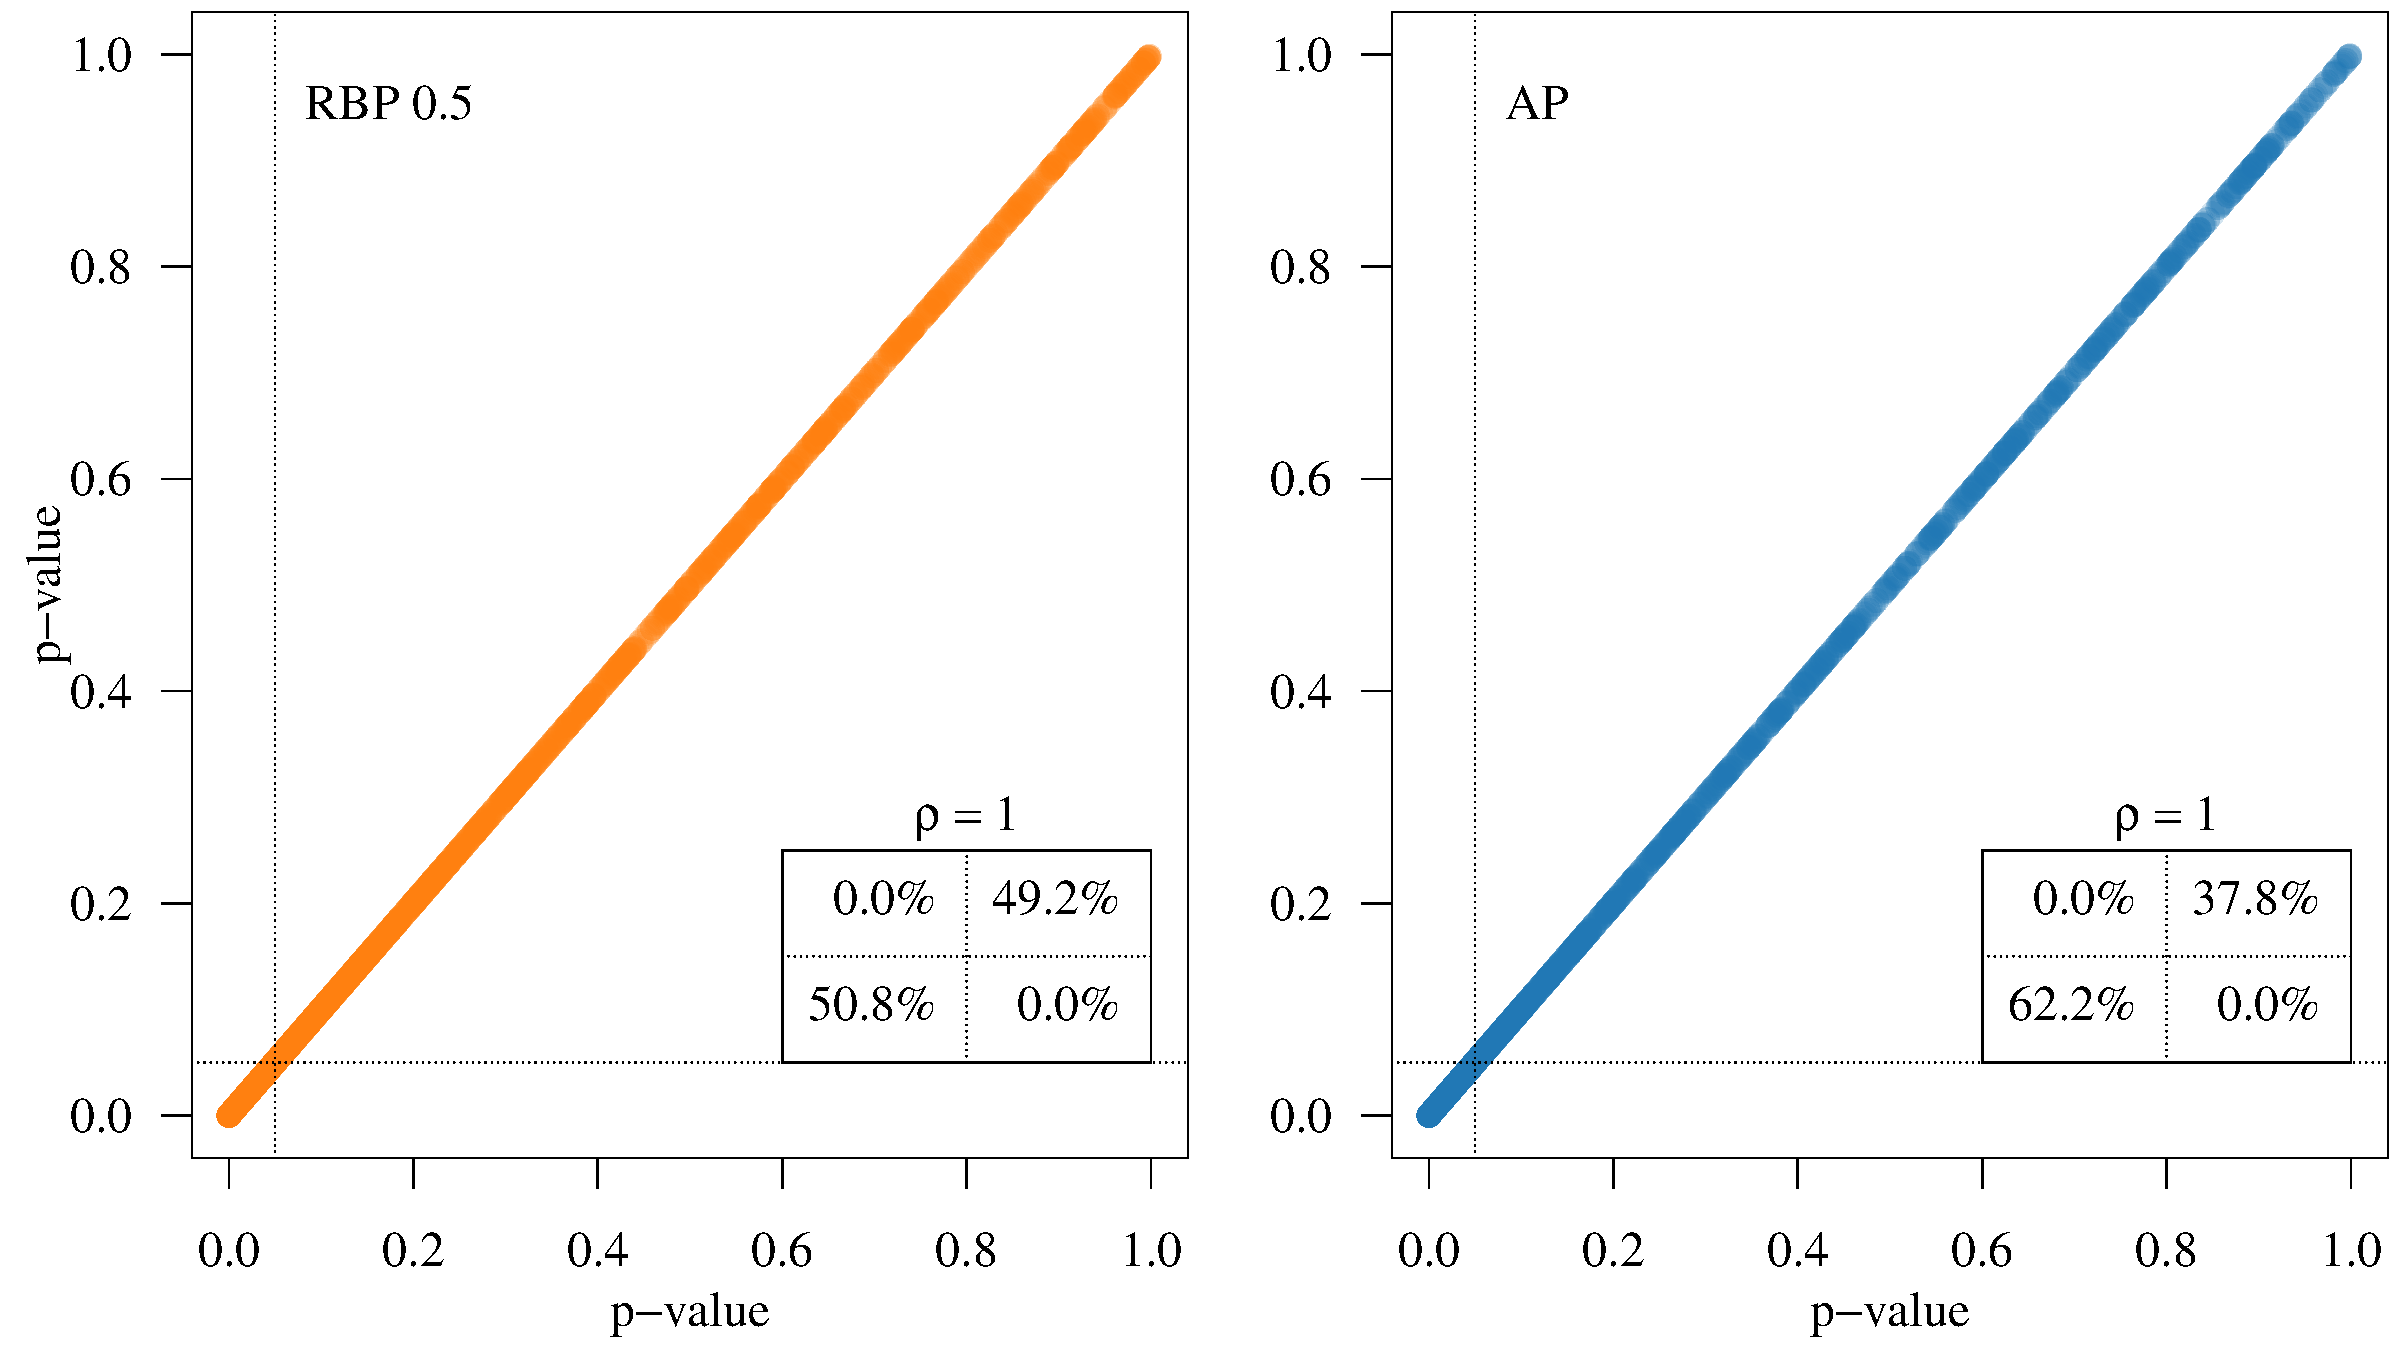
\includegraphics[width=0.98\textwidth, page=1]{figs/p_scatter_for_talk.pdf}
\end{frame}

\begin{frame}{Correlation of $p$ Values for All System Pairs}
\includegraphics[width=0.98\textwidth, page=3]{figs/p_scatter_for_talk.pdf}
\end{frame}

\begin{frame}{Correlation of $p$ Values for All System Pairs}
\includegraphics[width=0.98\textwidth, page=5]{figs/p_scatter_for_talk.pdf}
\end{frame}

\begin{frame}{Correlation of $p$ Values for All System Pairs}
\includegraphics[width=0.98\textwidth, page=6]{figs/p_scatter_for_talk.pdf}
\end{frame}

\begin{frame}{Correlation of $p$ Values for All System Pairs}
\includegraphics[width=0.98\textwidth, page=7]{figs/p_scatter_for_talk.pdf}
\end{frame}

\begin{frame}{Correlation of $p$ Values for All System Pairs}
\includegraphics[width=0.98\textwidth, page=11]{figs/p_scatter_for_talk.pdf}
\end{frame}

\begin{frame}{Summary}
Similarity score {\color{blue}ties} do have {\color{blue}potential} to affect system comparisons. But fortunately, {\color{blue}in practice}, they {\color{blue}did not}.\\[1.5em]

Allowing {\color{blue}deliberate introduction} of {\color{blue}ties} in runs by grouping rules resulted only {\color{blue}small changes} in the ability to {\color{blue}compare systems}. Reducing the accuracy of similarity scores to improve search speed and reduce space used is feasible.


\end{frame}

\begin{frame}{Thank You}
\Big{Question?}\\[5em]
\small{Acknowledgment: Thank AIRS and SIGIR for the student traveling scholarship.}
\end{frame} 

\end{document}


